\documentclass{amsart}

\usepackage[english]{babel}
\usepackage[utf8]{inputenc}
\usepackage{graphicx}
\usepackage{mathtools}
\usepackage{amsthm}
\usepackage{amsfonts}
\usepackage{hyperref}
\usepackage[singlelinecheck=false]{caption}
\usepackage[backend=biber,url=true,doi=true,eprint=false,style=alphabetic]{biblatex}
\usepackage{enumitem}
\usepackage[justification=centering]{caption}
\usepackage{indentfirst}
\usepackage{algorithm}
\usepackage{algpseudocode}

\addbibresource{references.bib}

\makeatletter
\def\subsection{\@startsection{subsection}{3}%
  \z@{.5\linespacing\@plus.7\linespacing}{.1\linespacing}%
  {\normalfont\itshape}}
\makeatother

\DeclareMathOperator*{\argmin}{arg\,min}
\DeclareMathOperator*{\argmax}{arg\,max}

\newcommand\defeq{\mathrel{\overset{\makebox[0pt]{\mbox{\normalfont\tiny\sffamily def}}}{=}}}

\algrenewcommand\algorithmicrequire{\textbf{Input}}
\algrenewcommand\algorithmicensure{\textbf{Output}}

\captionsetup[table]{labelsep=space}

\theoremstyle{plain}

\newtheorem*{definition}{Definition}
\newtheorem{theorem}{Theorem}
\newtheorem{proposition}{Proposition}
\newtheorem{exercise}{Exercise}

\newcommand{\set}[1]{\mathcal{#1}}
\newcommand{\pr}{\mathbb{P}}
\renewcommand{\implies}{\Rightarrow}

\setlength{\parskip}{1em}

\title[]{4. Markov Networks}
\author[]{Renato Lui Geh\\NUSP\@: 8536030}

\begin{document}

\begin{abstract}
  This document shows the solutions to the proposed exercises.
  \vspace*{-2.5em}
\end{abstract}

\maketitle

\section{Exercises}

\begin{exercise}
  Prove that the following statements are equivalent for two nodes $X$ and $Y$ in an acyclic
  directed graph $G$:

  \begin{enumerate}[label=\roman*]
    \item $X$ and $Y$ are adjacent.
    \item There is no set $\mathbf{Z}$ that d-separated $X$ and $Y$.
    \item $X$ and $Y$ are not d-separated by $An(X)\cup An(Y)$.
    \item $X$ and $Y$ are not d-separated by $Pa(X)\cup Pa(Y)$.
  \end{enumerate}
\end{exercise}

\begin{proof}
  Since $X$ and $Y$ are adjacent, than there exists an edge $X\rightarrow Y$ or $Y\rightarrow X$.
  From the definition of d-separation, we can conclude that $X$ and $Y$ are d-connected (or
  unblocked). This equates to saying states (i) and (ii). For statements (iii) and (iv), consider
  the following graphs:

  \begin{figure}[h]
    \centering{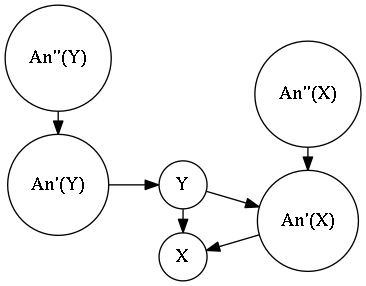
\includegraphics[scale=0.3]{graphs/ex1_a.png}
      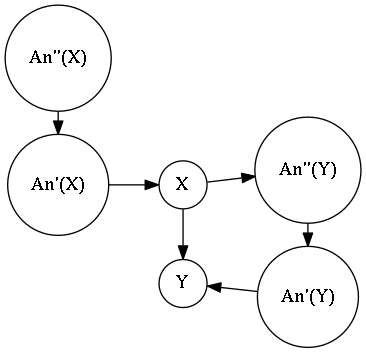
\includegraphics[scale=0.3]{graphs/ex1_b.png}
      \caption{Graph (a) on the left and graph (b) on the right.}
    }
  \end{figure}

  These two graphs summarize all possible situations in which the ancestrals of $X$ and $Y$ could
  be connected to $X$ and $Y$ respectively. Consider graph (a). Note that we cannot form any
  connection $(X,Y,An(X),An(Y))$ such that $X$ and $Y$ are d-separated. For instance, consider the
  path $Y\rightarrow An'(X)\rightarrow X$. In this case $An'(X)$ indeed blocks $X$ and $Y$; however
  there exists a path $Y\rightarrow X$ that is unblocked. From the definition of d-separation, if
  there exists an unblocked trail, then variables $X$ and $Y$ are not d-separated. This explains
  the equivalence of statement (iv). Now consider graph (b). Again, the path $X\rightarrow An'(Y)
  \rightarrow An''(y)\rightarrow Y$ is a serial connection where $\mathcal{B}=\{An'(Y),An''(Y)\}$
  blocks $X$ and $Y$. Similar to our previous conjecture, for $X$ and $Y$ to be d-separated all
  trails must be blocked. Yet, $X\rightarrow Y$ is obviously unblocked, proving that $X$ and $Y$
  must be d-connected.

  The resulting decisions are presented below:

  \begin{description}
    \item[] $B\perp C|A$?
      \begin{description}
        \item[true] $\implies$ Graph (1)
        \item[false] $\implies$ Graph (2) or (3)
        \item[] $B\perp C|\emptyset$?
          \begin{description}
            \item[true] Graph (3)
            \item[false] Graph (2)
          \end{description}
      \end{description}
  \end{description}
\end{proof}

\begin{exercise}
  Suppose you have an independency oracle $I$ which answers independency queries ``is
  $X\perp Y|Z$?''. Discuss how you can use the result in the previous exercise and the oracle to
  decide which of the graphs below represent the independency relation induced by the oracle. Make
  an effort to find the most computationally efficient way, that is, one which calls the oracle the
  least number of times.

  \begin{figure}[h]
    \centering{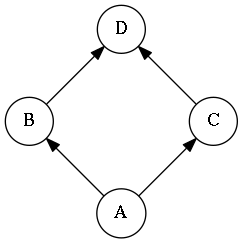
\includegraphics[scale=0.3]{graphs/ex2_q1.png}
      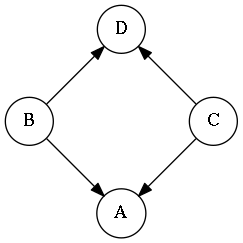
\includegraphics[scale=0.3]{graphs/ex2_q2.png}
      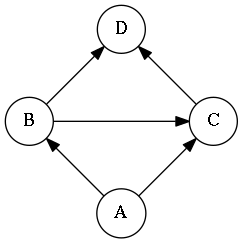
\includegraphics[scale=0.3]{graphs/ex2_q3.png}
      \caption{Possible graphs as solutions. Numbered 1 to 3 from left to right.}
    }
  \end{figure}
\end{exercise}

\begin{proof}[Solution]
  First we ask the query $I(B,A,C)$ (i.e. $B\perp C|A$) to the oracle. If the result is true, then
  we have that the corresponding graph is (1). Otherwise it may either be (2) or (3). This
  condition is true since, if the statement $I(B,A,C)$ is true, then $B$ and $C$ must be
  d-separated. For graph (1) we have two connections: convergent and divergent. Since we were given
  $A$, then both connections have $A$ block $B$ and $C$. Thus we conclude $B$ and $C$ are
  d-separated in graph (1). Graph (2) has two convergent connections: $B\to A\gets C$ and $B\to D
  \gets C$. We only have $A$ as evidence, so the first path is indeed unblocked; therefore, even
  though $B\to D\gets C$ is blocked, there still exists a trail that unblocks $B$ and $C$, making
  them d-separated. For graph (3) we have the trivial case where $B$ and $C$ are adjacent. From the
  previous exercise --- item (iv) --- we know that $B\not\perp C|A$.

  Now consider the query $I(B,\emptyset,C)$. Graph (2) has two convergent connections: $B\to A\gets
  C$ and $B\to D\gets C$. We were given no evidence, which means $B$ and $C$ are blocked on both
  trails, which means $I(B,\emptyset,C)=true$ in graph (2). $B$ and $C$ are adjacent in graph (3).
  From item (ii) of our previous exercise we know that there is no set $\mathbf{Z}$ in which $B$
  and $C$ are d-separated. Therefore $B\not\perp C|(\mathbf{Z}=\emptyset)\equiv I(B,\mathbf{Z}=
  \emptyset,C)=false$.
\end{proof}

\newpage

\printbibliography[]

\end{document}
